\documentclass{article}
\usepackage[utf8]{inputenc}
\usepackage{graphicx}
\usepackage{float} 

\title{Grupo Bimbo Inventory Demand \\Data Science Report }
\author{Juan Manuel Serrano Rodriguez, Nicolas Guevara Herran,\\ Giovanny Esteban Moreno Rondon}
\date{July 2024}

\begin{document}

\maketitle

\section{Gathering Data and Exploration}
\subsection{Kaggle and Web Scrapping}
The dataset for this competition was primarily sourced from Kaggle. Additionally, we utilized web scraping techniques to augment our data with external variables. Specifically, we collected biweekly inflation rates and consumer confidence indices from an API. These additional variables were gathered for the period from March 31st to June 1st, 2016.

\subsection{Data Exploration}

Initial data exploration involved understanding the structure and summary statistics of the dataset. Key columns include:

\begin{itemize}
    \item Week (Semana)
    \item Sales Depot ID (Agencia\_ID)
    \item Sales Channel ID (Canal\_ID)
    \item Route ID (Ruta\_SAK)
    \item Client ID (Cliente\_ID)
    \item Client Name (NombreCliente)
    \item Product ID (Producto\_ID)
    \item Product Name (NombreProducto)
    \item Sales Units This Week (Venta\_uni\_hoy)
    \item Sales This Week in Pesos (Venta\_hoy)
    \item Returns Units Next Week (Dev\_uni\_proxima)
    \item Returns Next Week in Pesos (Dev\_proxima)
    \item Adjusted Demand (Demanda\_uni\_equil)
\end{itemize}

Exploratory data analysis (EDA) was conducted to identify patterns, trends, and anomalies within the data. 

To understand the structure and characteristics of our dataset, we employed various graphical representations and utilized the YData Profile Report. This step helped us identify the distribution of our data, detect any anomalies, and gain insights into potential relationships between variables.

\begin{figure}[H]
\begin{center}
\centering
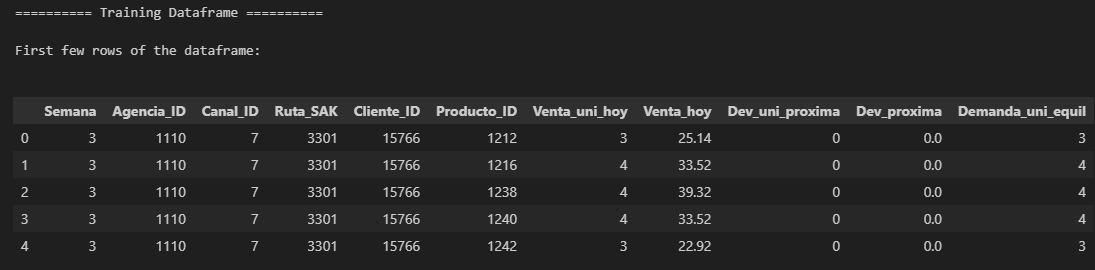
\includegraphics[width=0.9\textwidth]{images/train_df.png}
\caption{Train Dataframe}
\end{center}
\end{figure}

\begin{figure}[H] 
\begin{center}
\centering
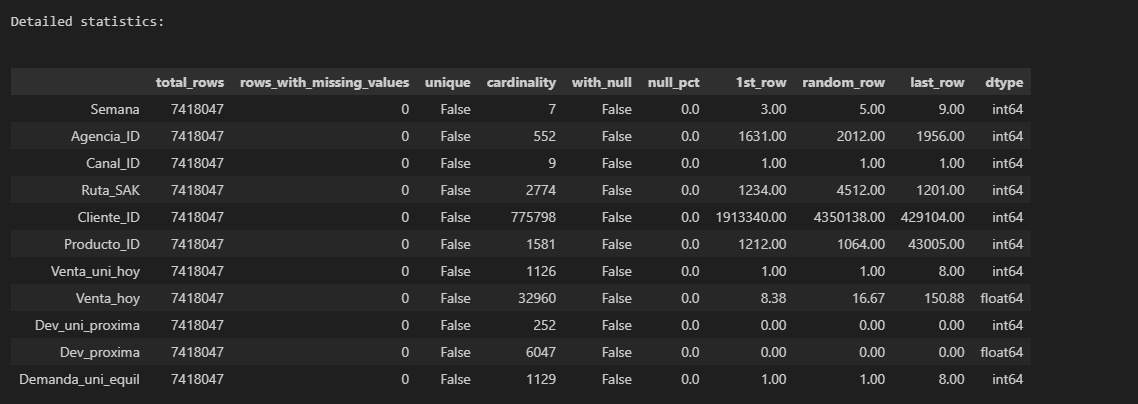
\includegraphics[width=0.9\textwidth]{images/descrip_train.png}
\caption{Description Train Dataframe}
\end{center}
\end{figure}

\begin{figure}[H]
\begin{center}
\centering
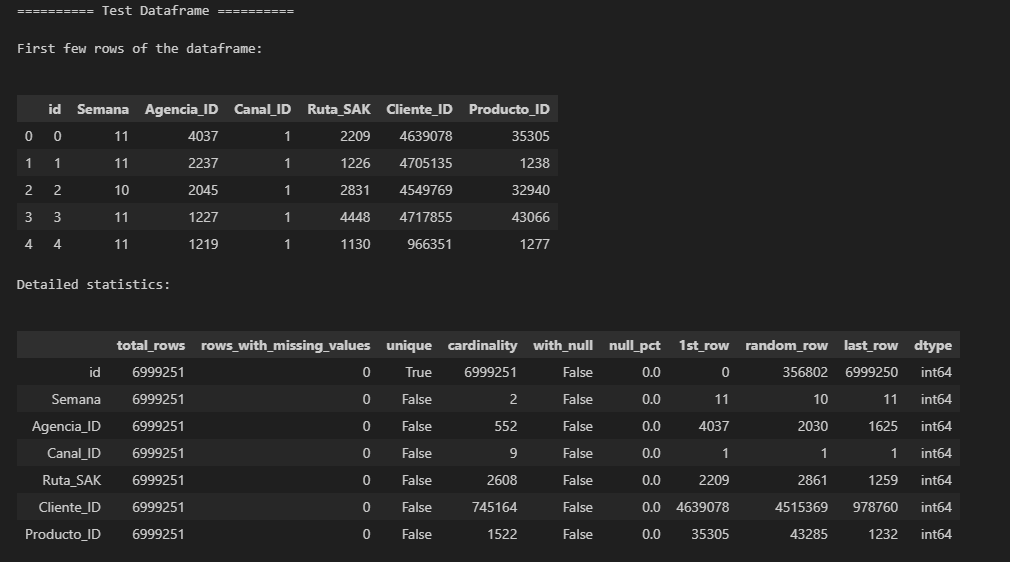
\includegraphics[width=0.9\textwidth]{images/test_df.png}
\caption{Test Dataframe}
\end{center}
\end{figure}

\begin{figure}[H] 
\begin{center}
\centering
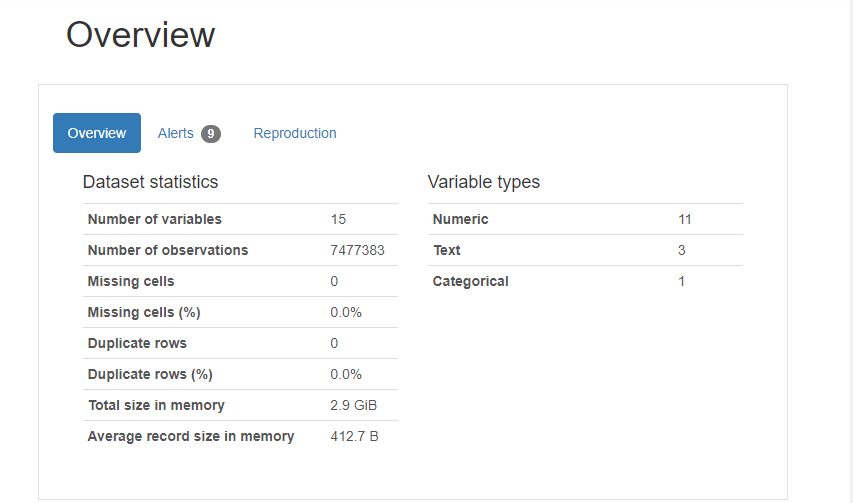
\includegraphics[width=0.9\textwidth]{images/train_ydata.png}
\caption{Ydata Profile Report Dataframe}
\end{center}
\end{figure}
    

\section{Data Preprocessing}
Data preprocessing is a critical step to ensure data quality and prepare it for modeling.
\begin{itemize}
    \item Data Cleaning: Missing values were handled, and duplicate records were removed. Outliers were identified and treated appropriately.
    \item Data Integration: The external economic indicators (bi-weekly inflation and consumer confidence index) were integrated with the primary dataset based on the corresponding time periods.
    \item Data Transformation: Features were transformed to appropriate data types to facilitate smooth pipeline operations.
\end{itemize}

\section{Feature Engineering}
Feature engineering involved creating new variables to capture additional information and improve model performance.
\begin{itemize}
    \item Temporal Features: Lagged variables were created to capture temporal dependencies in sales and demand.
    \item Economic Indicators: The bi-weekly inflation rate and consumer confidence index were added as features to capture the impact of economic conditions on product demand.
    \item Categorical Encoding: Categorical variables were converted to numerical format using one-hot encoding or label encoding.

\begin{figure}[H] 
    \begin{center}
    \centering
    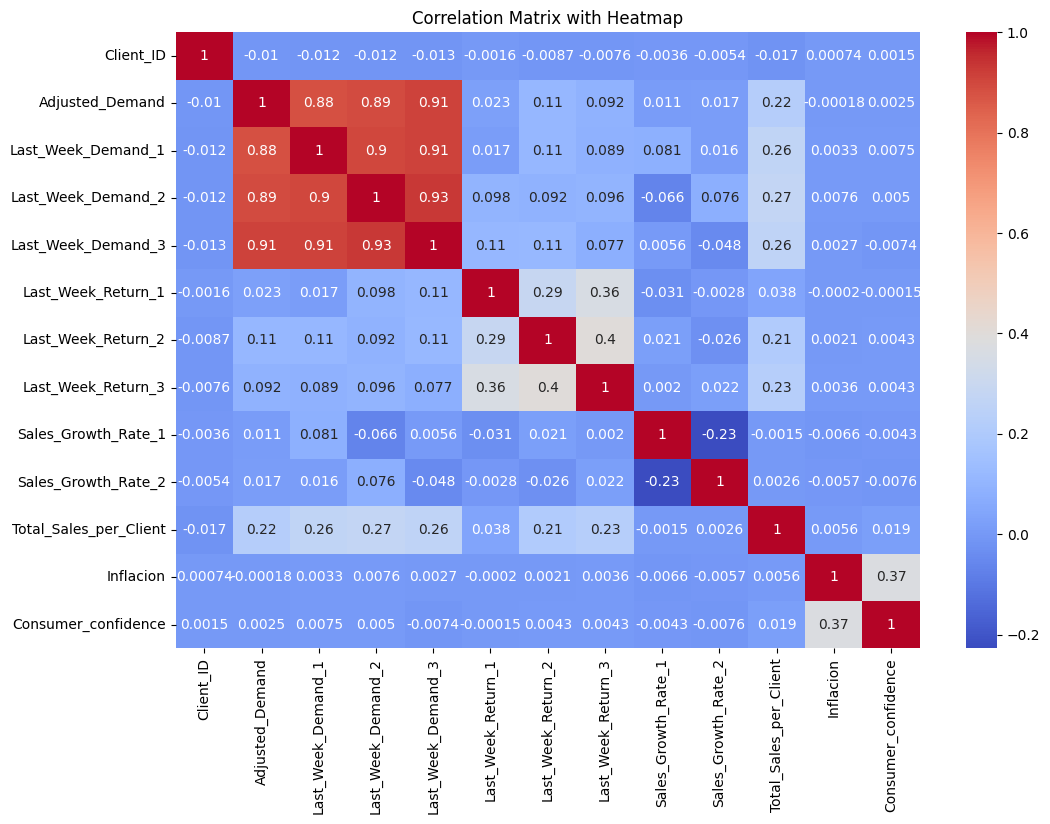
\includegraphics[width=0.9\textwidth]{images/output.png}
    \caption{Heatmap correlation of the features}
    \end{center}
\end{figure}    

\end{itemize}

\section{Model Selection}

Two machine learning models were selected for this study: XGBoost and Random Forest.
\begin{itemize}
    \item XGBoost: A gradient boosting framework known for its high performance and ability to handle complex interactions.
    \item Random Forest: An ensemble learning method that constructs multiple decision trees for improved robustness.
\end{itemize}

\section{Model Training}
The selected models were trained on the processed dataset.

\begin{itemize}
    \item $XGBoost$ Training: The XGBoost model was trained with parameters such as $n\_estimators=200$, $max\_depth=8$, $learning\_rate=0.2$, $subsample=0.9$, $colsample\_bytree=0.8$, $n\_jobs=-1$, and $random\_state=42$.
    \item $Random$ $Forest$ Training: The Random Forest model was trained with parameters including $n\_estimators=110$, $min\_samples\_split=10$, $min\_samples\_leaf=5$, $n\_jobs=-1$, and $random\_state=42$.
\end{itemize}

\section{Model Evaluation}
In this section, we evaluate and compare the performance of two machine learning models, Random Forest and XGBoost, on the task of predicting adjusted demand. We use metrics such as Mean Squared Error (MSE) and R-squared (R²) to assess the models' performance.
\begin{itemize}
    \item XGBoost Performance:
  
    \begin{figure}[H] 
        \begin{center}
        \centering
        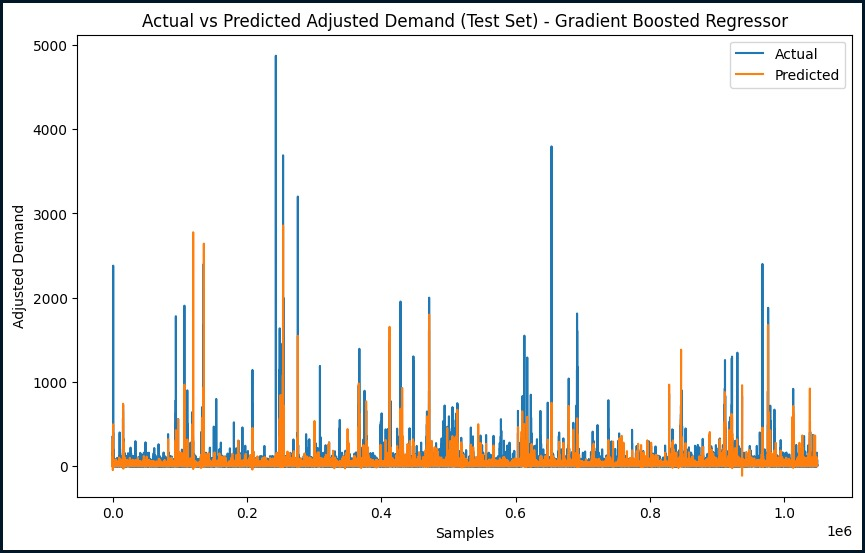
\includegraphics[width=0.8\textwidth]{images/comparisonxg.jpg}
        \caption{Heatmap correlation of the features}
        \end{center}
    \end{figure} 

    \item Random Forest Performance:
    
    \begin{figure}[H] 
        \begin{center}
        \centering
        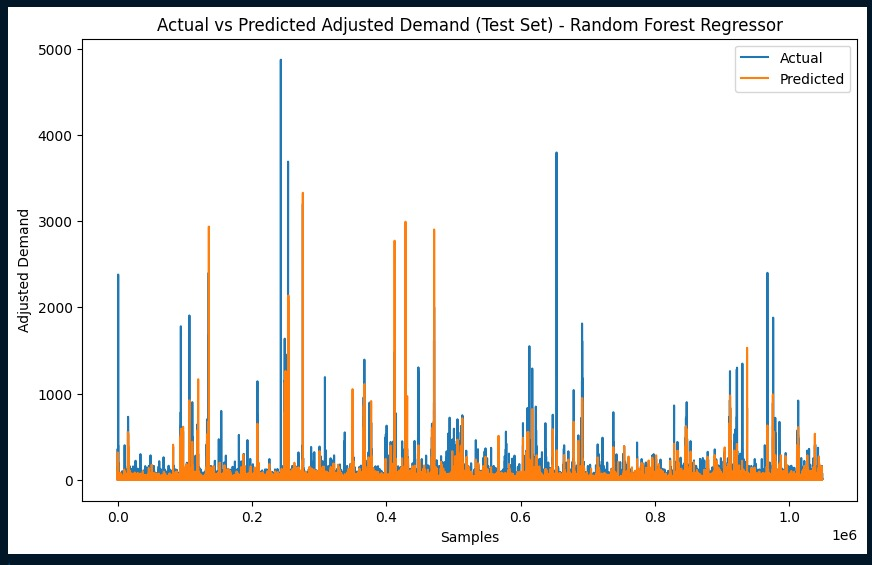
\includegraphics[width=0.8\textwidth]{images/comparison.jpg}
        \caption{Actual vs Predict Adjusted Demand}
        \end{center}
    \end{figure} 

\end{itemize}

\section{Business Questions}
The study aimed to address several business questions related to inventory management and demand forecasting:
\begin{itemize}
    \item What are our best customers per week?
    
    \begin{figure}[H] 
        \begin{center}
        \centering
        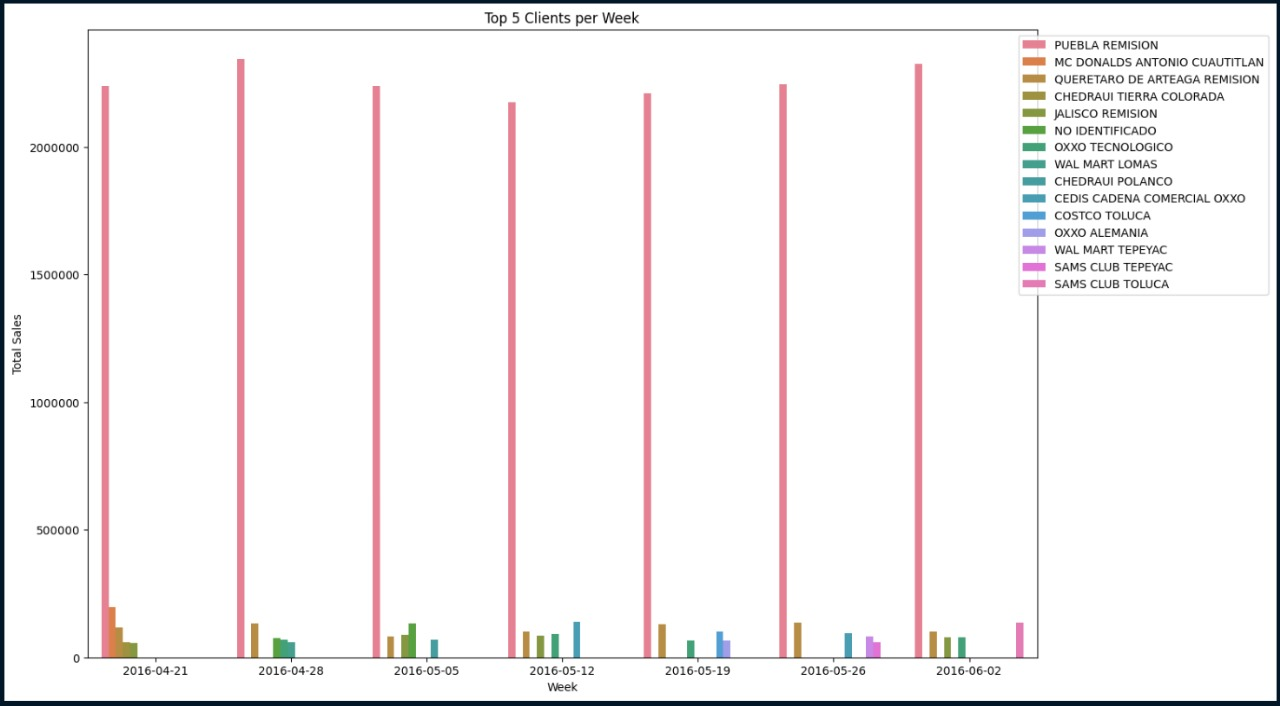
\includegraphics[width=0.8\textwidth]{images/question1.jpg}
        \caption{Business Question 1}
        \end{center}
    \end{figure} 

    \item What are the sales that WAL MART TEPEYAC had during the weeks? 

    \begin{figure}[H] 
        \begin{center}
        \centering
        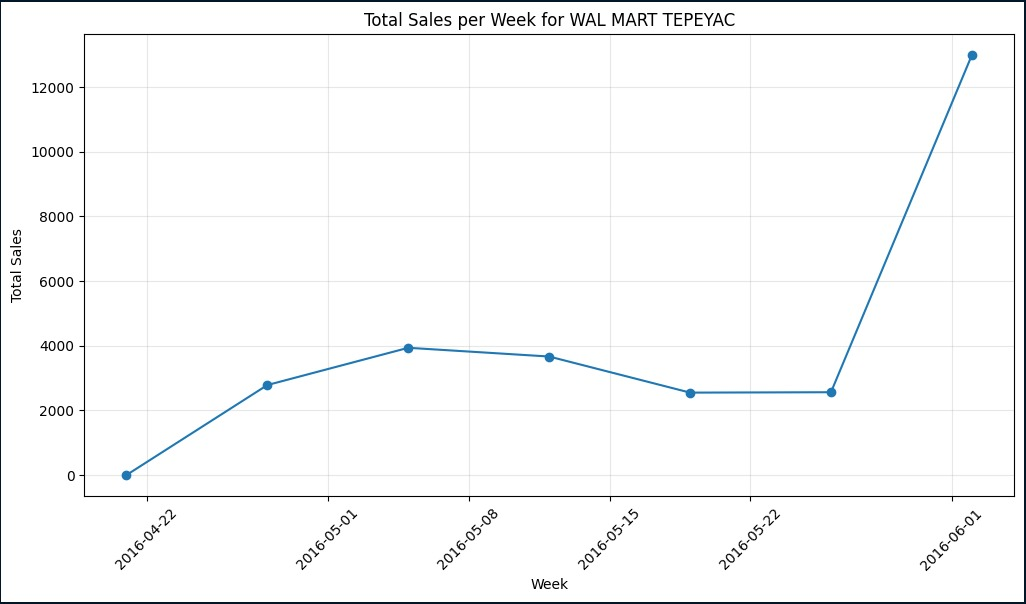
\includegraphics[width=0.8\textwidth]{images/question2.jpg}
        \caption{Business Question 2}
        \end{center}
    \end{figure} 

    \item How many sales and returns where done for each week?

    \begin{figure}[H] 
        \begin{center}
        \centering
        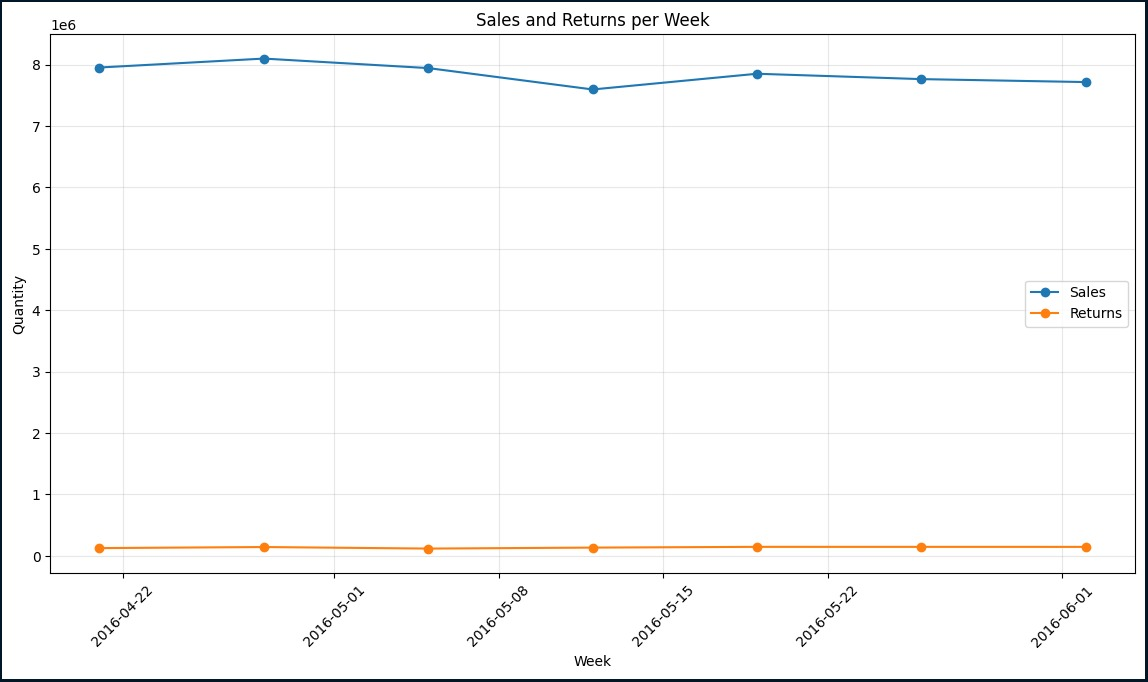
\includegraphics[width=0.7\textwidth]{images/question3.jpg}
        \caption{Business Question 3}
        \end{center}
    \end{figure}


    \item What are the top 10 products with most sales?

    \begin{figure}[H] 
        \begin{center}
        \centering
        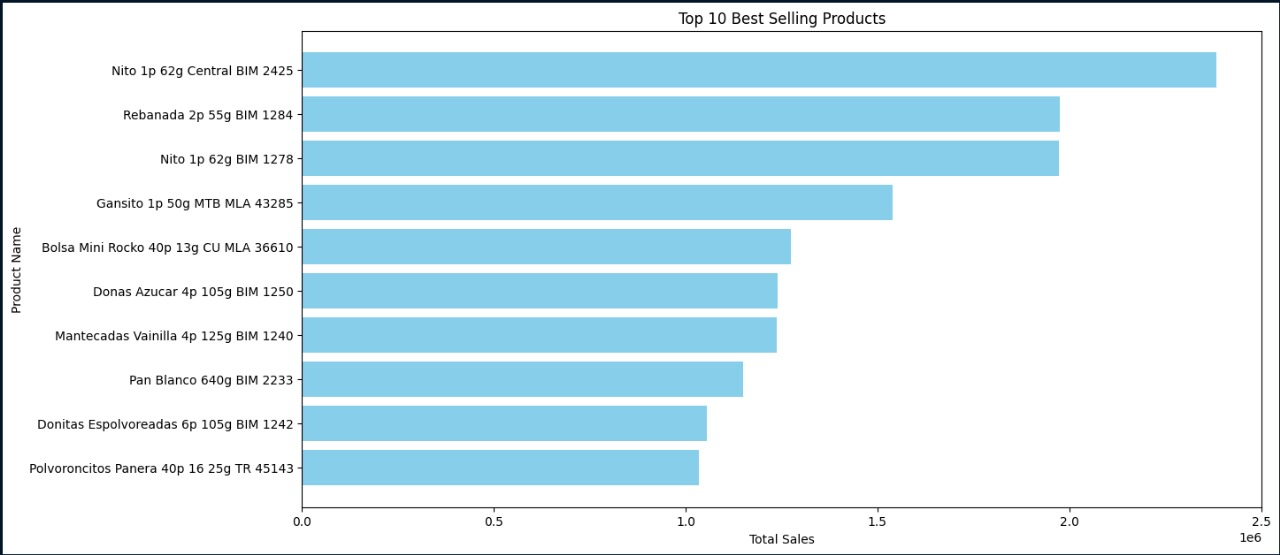
\includegraphics[width=0.8\textwidth]{images/question4.jpg}
        \caption{Business Question 4}
        \end{center}
    \end{figure}

    \item What are the states and towns where there have been more sales?

    \begin{figure}[H] 
        \begin{center}
        \centering
        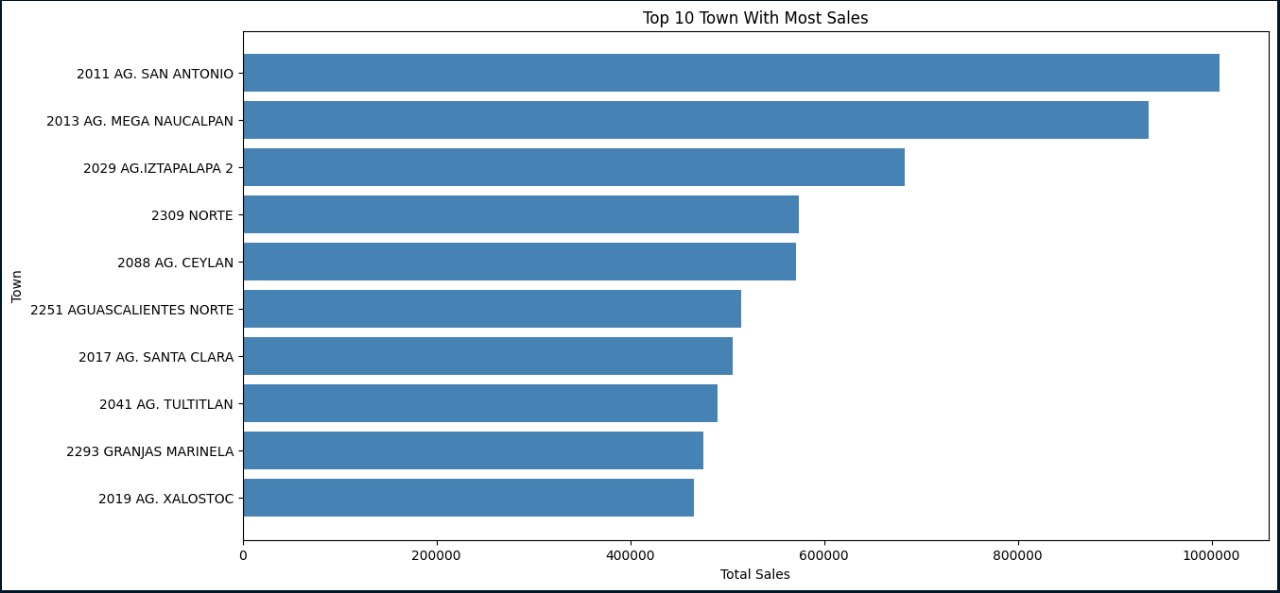
\includegraphics[width=0.8\textwidth]{images/question5.jpg}
        \caption{Business Question 5}
        \end{center}
    \end{figure}

\end{itemize}

\section{Conclusions}
This report demonstrates the application of machine learning models in forecasting product demand for Grupo Bimbo. The Random Forest model outperformed the XGBoost model, providing more accurate predictions of adjusted demand. The integration of external economic indicators, such as bi-weekly inflation rates and the consumer confidence index, significantly enhanced the model's accuracy. These findings highlight the potential of using advanced machine learning techniques to improve inventory management, reduce waste, and optimize resource allocation for Grupo Bimbo. Future work could involve incorporating additional features, such as macroeconomic indicators and weather data, to further enhance prediction accuracy.
\end{document}
